\documentclass[compress]{beamer}
\usepackage{irbookslide}
\usepackage{irilmenau2}
\usepackage{tikz}
\usepackage{url}
\usepackage{ifxetex}
%\RequireXeTeX
\usepackage{fontspec} % zahteva paket euenc
\usepackage{xunicode}
\usepackage{xltxtra}
\usepackage{polyglossia}
\usepackage{minted}
\usepackage{algorithmic}
\renewcommand{\algorithmicrequire}{\textbf{Input:}}
\renewcommand{\algorithmicensure}{\textbf{Output:}}
\usepackage{xcolor,colortbl}
\usepackage{textcomp}
%\setdefaultlanguage[script=Latin]{serbian}

\title{Python za Java programere}
\subtitle{izvor: http://python4java.necaiseweb.org}
\institute{Katedra za informatiku, Fakultet tehničkih nauka, Univerzitet u
Novom Sadu}
\date{2019.}
\subject{Predavanja sa OISISI}

\begin{document}

\frame{\titlepage}

\section{Uvod}
\begin{frame}[fragile]
  \frametitle{Python za Java programere}
  \begin{itemize}
    \item izvršavanje programa
    \item osnovne konstrukcije
    \item funkcije i metode
    \item interakcija sa korisnikom
    \item stringovi
    \item grananje i petlje
    \item funkcije
    \item moduli
    \item liste (nizovi)
    \item tekstualni fajlovi
    \item rečnici
    \item klase, veze među klasama
    \item preklapanje operatora
    \item izuzeci
    \item nasleđivanje
    \item kopiranje objekata
  \end{itemize}
\end{frame}

\begin{frame}[fragile]
\frametitle{Izvršavanje Python programa}

Python program je tekstualni fajl koji sadrži naredbe. Primer:

\begin{minted}[linenos=false]{python}
# Classic hello world program in Python.

print("Hello World")
print("How are you today?")
\end{minted}
\end{frame}

\begin{frame}[fragile]
\frametitle{Nema \texttt{main()}}

Prva naredba koja se izvršava je prva naredba u fajlu na globalnom nivou
(izvan svih funkcija i metoda).

U prethodnom primeru, to je prva \texttt{print} naredba.

\begin{minted}[linenos=false]{bash}
python myprogram.py
\end{minted}
\end{frame}

\begin{frame}[fragile]
\frametitle{Shebang za Linux i macOS}

Dodati kao prvi red u fajlu

\begin{minted}[linenos=false]{bash}
#!/usr/bin/python
\end{minted}

Zatim uključiti execute bit:

\begin{minted}[linenos=false]{bash}
chmod +x myprogram.py
\end{minted}

Nadalje se program može pokrenuti i ovako:

\begin{minted}[linenos=false]{bash}
./myprogram.py
\end{minted}  
\end{frame}

\begin{frame}[fragile]
\frametitle{Interaktivni mod}
Poziv Python interpretera:
\begin{minted}[linenos=false,fontsize=\footnotesize]{bash}
$ python
\end{minted}
\begin{minted}[linenos=false,fontsize=\footnotesize]{python}
Python 3.7.4 (default, Jul  9 2019, 18:13:23) 
[Clang 10.0.1 (clang-1001.0.46.4)] on darwin
Type "help", "copyright", "credits" or "license" for more information.
>>> x = 1
>>> y = x + 1
>>> y
2 
\end{minted}
\end{frame}

\section{Osnove}

\begin{frame}[fragile]
\frametitle{Osnovne konstrukcije}
Hello world u Javi:
\begin{minted}[linenos=false,fontsize=\small]{java}
// Hello World in Java.
public class HelloWorld {
  public static void main(String[] args) {
    System.out.println("Hello World");
  }
}
\end{minted}

Hello world u Pajtonu:

\begin{minted}[linenos=false,fontsize=\small]{python}
# Hello World in Python.
print("Hello World")
\end{minted}
\end{frame}

\begin{frame}[fragile]
\frametitle{Format reda}
\begin{itemize}
  \item naredba se ne završava sa tačka-zarez
  \item kraj linije je i kraj naredbe
\end{itemize}
\begin{minted}[linenos=false,fontsize=\small]{python}
print("Hello World!")
print("How are you today?")
\end{minted}

\begin{itemize}
  \item u Javi naredba se završava sa tačka-zarez i može se protezati kroz više
linija:
\end{itemize}
\begin{minted}[linenos=false,fontsize=\small]{java}
// Java statement
System.out.print
  (
    "Hello World!"
    )
;
\end{minted}
\end{frame}

\begin{frame}[fragile]
\frametitle{Format reda}
\begin{itemize}
  \item naredba se može protezati kroz više redova
  \item backslash za nastavak u sledećem redu
\end{itemize}
\begin{minted}[linenos=false,fontsize=\small]{python}
result = (someValue * 5 + anotherValue * 12) \
         - (originalValue * 2)
name = "John "\
       "Smith"
\end{minted}

\begin{itemize}
  \item poziv funkcija ima zagrade, pa se naredba ne mora nastavljati sa 
    backslash
\end{itemize}
\begin{minted}[linenos=false,fontsize=\small]{python}
myFunction(a, b,
           "name",
           avg)
\end{minted}
\end{frame}
  
\begin{frame}[fragile]
\frametitle{Komentari}
\begin{itemize}
  \item komentar počinje znakom hash i pruža se do kraja reda
  \item backslash za nastavak u sledećem redu
\end{itemize}
\begin{minted}[linenos=false,fontsize=\small]{python}
# This is a comment.
result = 0   # so is this
\end{minted}
\end{frame}
  
\begin{frame}[fragile]
\frametitle{Blok naredbi}
\begin{itemize}
  \item umesto vitičastih zagrada blok se definiše uvlačenjem redova
\end{itemize}
\begin{minted}[linenos=false,fontsize=\small]{python}
while i <= 20:
    total = total + i
    i = i + 1
print("The total =", total)
\end{minted}
\begin{itemize}
  \item ovakav primer u Javi glasio bi
\end{itemize}
\begin{minted}[linenos=false,fontsize=\small]{java}
while (i <= 20) {
  total = total + i;
  i = i + 1;
}
System.out.println("The total = " + total);
\end{minted}  
\end{frame}
  
\begin{frame}[fragile]
\frametitle{Uvlačenje naredbi}
\begin{itemize}
  \item naredbe iza kojih sledi blok imaju dvotačku na kraju
  \item samo naredbe u bloku mogu biti dodatno uvučene
  \item top-level naredbe ne smeju biti uvučene
\end{itemize}
\begin{itemize}
  \item nije važan broj razmaka prilikom uvlačenja
  \item važno je da su sve naredbe uvučene za isti broj razmaka
  \item prva naredba sa drugačijim uvlačenjem označava kraj bloka
  \item u interaktivnom modu, prazan red isto završava blok
\end{itemize}
\begin{itemize}
  \item preporuka iz PEP8: \textbf{uvlačenje za 4 razmaka}
  \item uvek razmak, nikad tab
\end{itemize}
\end{frame}

\begin{frame}[fragile]
\frametitle{Identifikatori}
\begin{itemize}
  \item case sensitive
  \item mogu da sadrže slova, cifre, underscore
  \item ne smeju početi cifrom
\end{itemize}
\begin{itemize}
  \item rezervisane reči
\end{itemize}
\begin{minted}[linenos=false,fontsize=\small]{python}
and     assert    break     class     continue
def     del       elif      else      except
exec    finally   for       from      global
if      import    in        is        lambda
not     or        pass      print     raise
return  try       while
\end{minted}
\end{frame}
  
\begin{frame}[fragile]
\frametitle{Identifikatori}
\begin{itemize}
  \item nazivi tipova i ugrađenih funkcija
  \item mogu se redefinisati
  \item ali to je loša ideja
\end{itemize}
\begin{minted}[linenos=false,fontsize=\small]{python}
float
int
str
sum
max
\end{minted}
\end{frame}
  
\begin{frame}[fragile]
\frametitle{Tipovi podataka}
\begin{itemize}
  \item svi tipovi podataka su objekti
  \item nema razlike između primitivnih tipova i objekata kao u Javi
\end{itemize}
\begin{minted}[linenos=false,fontsize=\small]{python}
x = 1
y = 2L  # samo u Python 2.x
z = "tralala"
p = 0.1
q = 1e-2  # 0.01
r = 3 + 4j
\end{minted}
\end{frame}
  
\begin{frame}[fragile]
\frametitle{Tipovi podataka}
\begin{tabular}{llp{7cm}}
  \textbf{Python 3} & \textbf{Java} & \textbf{napomena} \\ \hline
  \texttt{int} & \texttt{long} & \texttt{int} se uglavnom ponaša kao Java \texttt{long}, ali nema ograničenje na veličinu broja! \\ \hline
  \texttt{float} & \texttt{double} & 64-bitni IEEE 754 \\ \hline
  \texttt{complex} & --- & kompleksni brojevi \\ \hline
  \texttt{bool} & \texttt{boolean} & \texttt{True} ili \texttt{False} \\ \hline
  \texttt{str} & \texttt{String} & nepromenljivi nizovi karaktera, jednostruki ili dvostruki navodnici \\ \hline
  \texttt{list} & \texttt{T[]} & nizovi: auto-resize, heterogeni \\ \hline
  \texttt{tuple} & --- & niz koji se ne može menjati nakon kreiranja \\ \hline
  \texttt{dict} & --- & asocijativna mapa (rečnik) \\ \hline
  \texttt{set} & --- & neuređena kolekcija objekata, bez duplikata
\end{tabular}
\end{frame}
  
\begin{frame}[fragile]
\frametitle{Promenljive}
\begin{itemize}
  \item svi tipovi podataka su objekti
  \item čuvaju se reference na objekte
  \item nema deklaracije promenljivih; one se kreiraju prilikom prve dodele
\end{itemize}
\begin{minted}[linenos=false,fontsize=\small]{python}
name = "John Smith"
id = 42
avg = 3.45
\end{minted}
\begin{itemize}
  \item Java ekvivalent
\end{itemize}
\begin{minted}[linenos=false,fontsize=\small]{java}
String name = "John Smith";
int id = 42;
double avg = 3.45;
\end{minted}  
\end{frame}
    
\begin{frame}[fragile]
\frametitle{Promenljive}
\begin{itemize}
  \item promenljiva nema tip
  \item može čuvati referencu na bilo koji objekat
\end{itemize}
\begin{center}
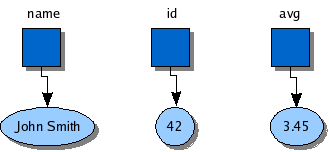
\includegraphics[scale=0.7]{variables.png}
\end{center}
\end{frame}
    
\begin{frame}[fragile]
\frametitle{Dodela vrednosti}
\begin{itemize}
  \item kada se nova referenca dodeli promenljivoj, stara referenca se gubi
\end{itemize}
\begin{minted}[linenos=false,fontsize=\small]{python}
id = 70
\end{minted}
\begin{center}
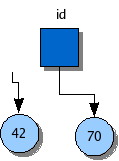
\includegraphics[scale=0.7]{newref.png}
\end{center}
\end{frame}
  
\begin{frame}[fragile]
\frametitle{Dodela vrednosti}
\begin{itemize}
  \item nova referenca može biti na objekat drugog tipa
\end{itemize}
\begin{minted}[linenos=false,fontsize=\small]{python}
id = "smith"
\end{minted}
\begin{center}
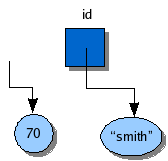
\includegraphics[scale=0.7]{diffref.png}
\end{center}
\end{frame}
  
\begin{frame}[fragile]
\frametitle{Konstante: ne postoje}
\begin{itemize}
  \item dve konstante u Javi
\end{itemize}
\begin{minted}[linenos=false,fontsize=\small]{java}
final double TAX_RATE = 0.06;
final int MAX_SIZE = 100;
\end{minted}
\begin{itemize}
  \item konvencija za promenljive kojima nećemo menjati vrednost: uppercase
\end{itemize}
\begin{minted}[linenos=false,fontsize=\small]{python}
TAX_RATE = 0.06
MAX_SIZE = 100
\end{minted}
\end{frame}

\begin{frame}[fragile]
\frametitle{Aritmetički operatori}
\begin{tabular}{lp{5cm}}
  \textbf{operator} & \textbf{napomena} \\ \hline
  \texttt{+} & sabiranje \\ \hline
  \texttt{-} & oduzimanje \\ \hline
  \texttt{*} & množenje \\ \hline
  \texttt{/} & deljenje \\ \hline
  \texttt{**} & stepenovanje \\ \hline
  \texttt{//} & celobrojno deljenje \\ \hline
  \texttt{\%} & ostatak
\end{tabular}
\begin{itemize}
  \item ima \texttt{+=}, \texttt{-=}, \dots
  \item nema \texttt{++} i \texttt{--}
\end{itemize}
\end{frame}
    
\begin{frame}[fragile]
\frametitle{Mešanje numeričkih tipova: \texttt{1 + 2.0}}
\begin{itemize}
  \item operand manjeg ranga se konvertuje u veći rang
  \item rang tipova: \\
    \texttt{complex} > \texttt{float} > \texttt{int}
\end{itemize}
\end{frame}
    
\begin{frame}[fragile]
\frametitle{Konverzija tipova}
\begin{itemize}
  \item automatska konverzija samo za numeričke tipove unutar numeričkih izraza
  \item sve ostale konverzije moraju biti eksplicitne
\end{itemize}
\begin{minted}[linenos=false,fontsize=\small]{python}
x = 100
y = "abc"
z = y + str(x)
\end{minted}
\end{frame}

\begin{frame}[fragile]
\frametitle{Glavni program i Java}
\begin{minted}[linenos=false,fontsize=\small]{java}
// Sumation.java
// Compute the sum of the first 100 integer values and print
// the results.
public class Summation {
  public static void main(String[] args) {
    final int NUM_VALUES = 100;
    int summation = 0;
    int i = 0;

    while (i <= NUM_VALUES) {
      summation = summation + 1;
      i = i + 1;
    }

    System.out.println("The sum of the first " + NUM_VALUES
                        + " integers is " +  summation);
  }
}
\end{minted}
\end{frame}
  
\begin{frame}[fragile]
\frametitle{Glavni program i Python}
\begin{minted}[linenos=false,fontsize=\small]{python}
# summation.py
# Compute the sum of the first 100 integer values and print
# the results.

# Initialize a constant variable.
NUM_VALUES = 100

# Compute the sum.
summation = 0
i = 1
while i <= NUM_VALUES:
   summation = summation + i
   i = i + 1

# Print the results.
print("The sum of the first", NUM_VALUES,
      "integers is", summation)
\end{minted}
\end{frame}
  
\section{Funkcije}

\begin{frame}[fragile]
\frametitle{Funkcija}
\begin{itemize}
  \item slična \texttt{static} metodi u Javi
  \item koriste se nezavisno od objekata
  \item u Pajtonu se ne definišu unutar klase
  \item (ali i mogu)
\end{itemize}
\begin{minted}[linenos=false,fontsize=\small]{python}
x = 100
y = "abc"
z = y + str(x)
\end{minted}
\end{frame}
  
\begin{frame}[fragile]
\frametitle{Ugrađene funkcije}
\begin{itemize}
  \item neke funkcije su deo jezika kao ugrađene (built-in)
  \item uvek su dostupne
\end{itemize}
\begin{minted}[linenos=false,fontsize=\small]{python}
# Compute the absolute value of the integer x
y = abs(x)
\end{minted}
\end{frame}
  
\begin{frame}[fragile]
\frametitle{Prenos parametara}
\begin{itemize}
  \item parametri funkcije se uvek prenose \textbf{po referenci}
  \item više parametara se razdvaja zarezom
  \item nema navođenja tipova parametara
\end{itemize}
\begin{itemize}
  \item mora se paziti da se prilikom poziva prosledi odgovarajući tip
  \item funkcije se mogu napisati i tako da primaju parametre različitog tipa
\end{itemize}
\end{frame}
  
\begin{frame}[fragile]
\frametitle{Rezultat funkcije}
\begin{itemize}
  \item rezultat je uvek referenca na objekat
  \item ili \texttt{None}
  \item ako se ne navede rezultat funkcije, podrazumevano se vraća \texttt{None}
\end{itemize}
\end{frame}

\section{Moduli}

\begin{frame}[fragile]
\frametitle{Pojam modula}
\begin{itemize}
  \item standardna biblioteka sadrži funkcije i klase organizovane u \textbf{module}
  \item modul je fajl sa Pajton kodom
  \item definicije iz drugog Pajton fajla (modula) možemo koristiti pomoću \texttt{import} naredbe
\end{itemize}
\begin{minted}[linenos=false,fontsize=\small]{python}
from math import *
y = sqrt(x)
\end{minted}
\begin{itemize}
  \item kod Jave konvencija je: jedna klasa -- jedan fajl
  \item kod Pajtona to ne mora biti tako
\end{itemize}
\end{frame}

\begin{frame}[fragile]
\frametitle{Import iz modula}
\begin{itemize}
  \item možemo importovati pojedinačne komponente iz modula
\end{itemize}
\begin{minted}[linenos=false,fontsize=\small]{python}
from math import sqrt
y = sqrt(x)
\end{minted}
\begin{itemize}
  \item možemo importovati ceo modul
  \item njegove komponente navodimo uz ime modula
\end{itemize}
\begin{minted}[linenos=false,fontsize=\small]{python}
import random
z = random.randrange(0, 10)
\end{minted}
\end{frame}
  
\begin{frame}[fragile]
\frametitle{Modul \texttt{math}}
\begin{tabular}{lp{5cm}}
  \textbf{funkcija} & \textbf{opis} \\ \hline
  \texttt{ceil(x)} & najmanji ceo broj veći od x \\ \hline
  \texttt{floor(x)} & najveći ceo broj manji od x \\ \hline
  \texttt{sqrt(x)} & kvadratni koren od x \\ \hline
  \texttt{sin(x)}, \texttt{cos(x)}, \texttt{tan(x)} & trigonometrijske funkcije \\ \hline
  \texttt{degrees(x)} & pretvara radijane u stepene \\ \hline
  \texttt{radians(x)} & pretvara stepene u radijane \\ \hline
  ... & ...
\end{tabular}
\end{frame}
  
\begin{frame}[fragile]
\frametitle{Import iz modula}
\begin{itemize}
  \item klasa predstavlja klasu objekata
  \item objekti su instance klase
  \item objekti se mogu upotrebiti nakon kreiranja
  \item svi literali u Pajtonu rezultuju kreiranim objektima
\end{itemize}
\begin{itemize}
  \item za kreiranje objekta direktno od klase, poziva se konstruktor kao da je nezavisna funkcija
\end{itemize}
\begin{minted}[linenos=false,fontsize=\small]{python}
from datetime import date
today = date(2019, 10, 1)
\end{minted}
\begin{itemize}
  \item kada se objekat kreira možemo pozivati njegove metode
\end{itemize}
\begin{minted}[linenos=false,fontsize=\small]{python}
whichDay = today.weekday()
\end{minted}
\end{frame}

\begin{frame}[fragile]
\frametitle{Konstruktori za numeričke tipove}
\begin{itemize}
  \item numerički tipovi imaju konstruktore za kreiranje objekata
  \item mogu poslužiti i za konverziju tipova
\end{itemize}
\begin{tabular}{lp{7cm}}
  \textbf{konstruktor} & \textbf{opis} \\ \hline
  \texttt{complex(x, y)} & kreira \texttt{complex} objekat, x i y moraju biti numerički tipovi \\ \hline
  \texttt{float(x)} & konvertuje string ili numerički tip u \texttt{float} \\ \hline
  \texttt{int(x)} & konvertuje string ili numerički tip u \texttt{int} \\ \hline
\end{tabular}
\end{frame}

\section[UI]{Interakacija sa korisnikom}

\begin{frame}[fragile]
\frametitle{Standardni ulaz}
\begin{minted}[linenos=false,fontsize=\small]{java}
// Java example
Scanner keyboard = new Scanner(System.in);
System.out.println("What is your name? ");
String name = keyboard.next();
\end{minted}

\ %

\begin{minted}[linenos=false,fontsize=\small]{python}
# Python example
name = input("What is your name? ")
\end{minted}
\end{frame}

\begin{frame}[fragile]
\frametitle{Unos numeričkih podataka}
\begin{minted}[linenos=false,fontsize=\small]{java}
// Java sample
System.out.print("What is your GPA?");
double gpa = keyboard.nextDouble();
\end{minted}

\ %

\begin{minted}[linenos=false,fontsize=\small]{python}
# Python example
gpa = float(input("What is your GPA? "))
\end{minted}
\end{frame}

\begin{frame}[fragile]
\frametitle{Standardni izlaz}
\begin{minted}[linenos=false,fontsize=\small]{python}
avg = grade / 3.0
print(avg)
\end{minted}

Funkcija \texttt{print} može primiti više parametara:

\begin{minted}[linenos=false,fontsize=\small]{python}
print("Your average grade =", avg)
\end{minted}

Funkcija \texttt{print} ne mora završiti ispis prelaskom u novi red:

\begin{minted}[linenos=false,fontsize=\small]{python}
print("Your average grade = ", end='')
print(avg)
\end{minted}
\end{frame}

\begin{frame}[fragile]
\frametitle{Primer programa (Java)$_1$}
\begin{minted}[linenos=false,fontsize=\footnotesize]{java}
/* Wages.java
 * Computes the taxes and wages for an employee given the
 * number of hours worked and their pay rate.
*/
import java.util.*;
public class Wages {
   public static void main(String[] args) {
      final double STATE_TAX_RATE = 0.035;
      final double FED_TAX_RATE = 0.15;
      double hours, payRate;
      double wages, stateTaxes, fedTaxes, takeHome;
      String employee;
      Scanner keyboard = new Scanner( System.in );
      System.out.print( "Employee name: " );
      employee = keyboard.next();
      System.out.print( "Hours worked: " );
      hours = keyboard.nextDouble();
      System.out.print( "Pay rate: " );
      payRate = keyboard.nextDouble();
\end{minted}
\end{frame}

\begin{frame}[fragile]
\frametitle{Primer programa (Java)$_2$}
\begin{minted}[linenos=false,fontsize=\footnotesize]{java}
      wages = hours * payRate;
      stateTaxes = wages * STATE_TAX_RATE;
      fedTaxes = wages * FED_TAX_RATE;
      takeHome = wages - stateTaxes - fedTaxes;
      System.out.println( "PAY REPORT" );
      System.out.println( "Employee: " + employee );
      System.out.println( "----------------------------------" );
      System.out.println( "Wages:       " + wages );
      System.out.println( "State Taxes: " + stateTaxes );
      System.out.println( "Fed Taxes:   " + fedTaxes );
      System.out.println( "Pay:         " + takeHome );
   }
}
\end{minted}
\end{frame}

\begin{frame}[fragile]
\frametitle{Primer programa (Python)}
\begin{minted}[linenos=false,fontsize=\footnotesize]{python}
# wages.py
# Computes the taxes and wages for an employee given the
# number of hours worked and their pay rate.
STATE_TAX_RATE = 0.035
FED_TAX_RATE = 0.15
employee = input("Employee name: ")
hours = float(input("Hours worked: "))
payRate = float(input("Pay rate: "))
wages = hours * payRate
stateTaxes = wages * STATE_TAX_RATE
fedTaxes = wages * FED_TAX_RATE
takeHome = wages - stateTaxes - fedTaxes
print "PAY REPORT"
print "Employee: ", employee
print "----------------------------------"
print "Wages:       ", wages
print "State Taxes: ", stateTaxes
print "Fed Taxes:   ", fedTaxes
print "Pay:         ", takeHome
\end{minted}
\end{frame}

\section[String]{Stringovi}

\begin{frame}[fragile]
\frametitle{Stringovi}
\begin{itemize}
  \item stringovi su instance klase \texttt{str}
  \item literal predstavlja referencu na objekat u memoriji
\end{itemize}
\begin{minted}[linenos=false,fontsize=\small]{python}
'string'
"string's"
\end{minted}

Pojavljivanje literala je kao poziv konstruktora. Sledeća dva reda daju isti 
rezultat.

\begin{minted}[linenos=false,fontsize=\small]{python}
name = "John Smith"
name = str('John Smith')
\end{minted}
\end{frame}

\begin{frame}[fragile]
\frametitle{Konverzija u string}
\begin{itemize}
  \item string konstruktor se može upotrebiti i za konverziju tipova
\end{itemize}
\begin{minted}[linenos=false,fontsize=\small]{python}
x = 45
intStr = str(x)          # '45'
floatStr = str(56.89)    # '56.89'
boolStr = str(False)     # 'False'
\end{minted}
\end{frame}

\begin{frame}[fragile]
\frametitle{Escape sekvence}
\begin{itemize}
  \item vrlo slično kao u Javi
\end{itemize}
\begin{minted}[linenos=false,fontsize=\small]{python}
msg = 'Start a newline here.\nusing the \\n character.'
\end{minted}
\begin{tabular}{lp{7cm}}
  \textbf{sekvenca} & \textbf{rezultat} \\ \hline
  \texttt{\textbackslash\textbackslash} & backslash (\textbackslash ) \\ \hline
  \texttt{\textbackslash'} & jednostruki navodnik (') \\ \hline
  \texttt{\textbackslash"} & dvostruki navodnik (") \\ \hline
  \texttt{\textbackslash n} & line feed karakter (LF, 10) \\ \hline
  \texttt{\textbackslash t} & tab karakter (HT, 9)
\end{tabular}
\end{frame}

\begin{frame}[fragile]
\frametitle{Višelinijski stringovi}
\begin{itemize}
  \item čuva se sav whitespace
\end{itemize}
\begin{minted}[linenos=false,fontsize=\small]{python}
"""This is a string which
can continue onto a new line. When printed, it will appear
   exactly as written between the trip quotes.
"""
\end{minted}
\begin{minted}[linenos=false,fontsize=\small]{python}
'''Here is another
        multiline string example 
     using triple single quotes.'''
\end{minted}
\end{frame}

\begin{frame}[fragile]
\frametitle{Konkatenacija}
\begin{minted}[linenos=false,fontsize=\small]{python}
strvar = 'This is '
fullstr = strvar + "a string"
\end{minted}
\begin{itemize}
  \item nema automatske konverzije tipova u string prilikom konkatenacije
\end{itemize}
\begin{minted}[linenos=false,fontsize=\small]{python}
result = "The value of x is " + str(x)
\end{minted}
\begin{itemize}
  \item konkatenacija može i bez operatora ako su dva stringa jedan do drugog
\end{itemize}
\begin{minted}[linenos=false,fontsize=\small]{python}
print("These two string literals " "will be concatenated.")
\end{minted}
\end{frame}

\begin{frame}[fragile]
\frametitle{Dužina stringa}
\begin{minted}[linenos=false,fontsize=\small]{java}
// Java string length
System.out.println("Length of the string = " + name.length());
\end{minted}

\ %

\begin{minted}[linenos=false,fontsize=\small]{python}
# Python string length
print("Length of the string =", len(name))
\end{minted}
\end{frame}

\begin{frame}[fragile]
\frametitle{Pristup znakovima u stringu po indeksu}
\begin{minted}[linenos=false,fontsize=\small]{java}
// Java character access
String msg = "This is a string";
System.out.println( "The first character is " +
                    msg.charAt( 0 ) );
System.out.println( "The last characater is " +
                    msg.charAt( msg.length() - 1 ) );
\end{minted}

\ %

\begin{minted}[linenos=false,fontsize=\small]{python}
# Python character access
msg = "This is a string!"
print("The first character is", msg[0])
print("The last character is", msg[len(msg) - 1])
\end{minted}
\end{frame}

\begin{frame}[fragile]
\frametitle{Negativni indeksi u nizu}
\begin{minted}[linenos=false,fontsize=\small]{python}
# poslednji znak u stringu
print("The last character is", msg[-1])
\end{minted}
\begin{center}
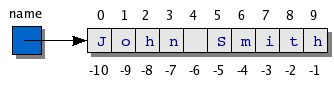
\includegraphics[scale=0.7]{strindex.png}
\end{center}
\end{frame}

\begin{frame}[fragile]
\frametitle{Podstringovi}
\begin{minted}[linenos=false,fontsize=\small]{java}
// Java substring extraction
String name = "John Smith";
String first = name.substring(0, 4);  // "John"
String last = name.substring(5);      // "Smith"
\end{minted}

Operator isecanja (\textit{slicing}) u Pajtonu postiže isti rezultat:

\begin{minted}[linenos=false,fontsize=\small]{python}
# Python substring extraction using slicing
name = "John Smith"
first = name[0:4]
last = name[5:]
\end{minted}
\end{frame}

\begin{frame}[fragile]
\frametitle{Umnožavanje stringova}
\begin{minted}[linenos=false,fontsize=\small]{python}
print("---------------------------------------------")
\end{minted}

je isto što i

\begin{minted}[linenos=false,fontsize=\small]{python}
print("-" * 45)
\end{minted}
\end{frame}

\begin{frame}[fragile]
\frametitle{Formatiranje stringa}
\begin{itemize}
  \item operator ostatka (\%) je definisan za stringove
  \item kreira novi string nalik \texttt{printf} metodi u Javi
\end{itemize}
\begin{minted}[linenos=false,fontsize=\small]{python}
output = "The average grade = %5.2f" % avgGrade
print(output)
\end{minted}
\begin{itemize}
  \item može i sa više vrednosti
\end{itemize}
\begin{minted}[linenos=false,fontsize=\small]{python}
print("Origin: (%d, %d)\n" % (pointX, pointY))
\end{minted}
\end{frame}

\begin{frame}[fragile]
\frametitle{Formatiranje stringa}
opšta struktura formata je
\begin{minted}[linenos=false,fontsize=\small]{text}
%[flags][width][.precision]code
\end{minted}

\ %

\begin{tabular}{lp{7cm}}
  \textbf{segment} & \textbf{opis} \\ \hline
  \texttt{flags} & vodeće nule (0) i poravnanje po levoj (-) ili desnoj (+) ivici \\ \hline
  \texttt{width} & broj znakova za prikaz \\ \hline
  \texttt{precision} & broj decimala \\ \hline
  \texttt{code} & specifikacija formata
\end{tabular}
\end{frame}

\begin{frame}[fragile]
\frametitle{Format specifier}
\begin{tabular}{lp{7cm}}
  \textbf{kod} & \textbf{opis} \\ \hline
  \texttt{\%s} & string ili drugi objekat \\ \hline
  \texttt{\%c} & karakter (iz ASCII vrednosti) \\ \hline
  \texttt{\%d} & celobrojna vrednost \\ \hline
  \texttt{\%i} & celobrojna vrednost (isto kao \texttt{\%d}) \\ \hline
  \texttt{\%u} & neoznačeni ceo broj \\ \hline
  \texttt{\%o} & oktalni ceo broj \\ \hline
  \texttt{\%x} & heksadecimalni ceo broj \\ \hline
  \texttt{\%X} & kao \texttt{\%x} samo uppercase \\ \hline
  \texttt{\%e} & float sa eksponentom \\ \hline
  \texttt{\%E} & kao \texttt{\%e} samo uppercase \\ \hline
  \texttt{\%f} & float bez eksponenta \\ \hline
  \texttt{\%g} & isto kao \texttt{\%e} ili \texttt{\%f} \\ \hline
  \texttt{\%G} & kao \texttt{\%g} samo uppercase \\ \hline
  \texttt{\%\%} & literal \texttt{\%}
\end{tabular}
\end{frame}

\begin{frame}[fragile]
\frametitle{Primer sa formatiranjem stringova}
\begin{minted}[linenos=false,fontsize=\footnotesize]{python}
# Computes the taxes and wages for an employee given the
# number of hours worked and their pay rate. The results
# are printed using formatted strings.
STATE_TAX_RATE = 0.035
FED_TAX_RATE = 0.15
employee = input("Employee name: ")
hours = float(input("Hours worked: "))
payRate = float(input("Pay rate: "))
wages = hours * payRate
stateTaxes = wages * STATE_TAX_RATE
fedTaxes = wages * FED_TAX_RATE
takeHome = wages - stateTaxes - fedTaxes
print("PAY REPORT")
print("Employee: %s" % employee)
print("----------------------------------")
print("Wages:       %8.2f" % wages)
print("State Taxes: %8.2f" % stateTaxes)
print("Fed Taxes:   %8.2f" % fedTaxes)
print("Pay:         %8.2f" % takeHome)
\end{minted}
\end{frame}




\end{document}